\begin{frame}{Simulated ``particles'' evolve to approximate posterior}
  \vspace{-0.2cm}
  \begin{tikzpicture}
    \node (a) {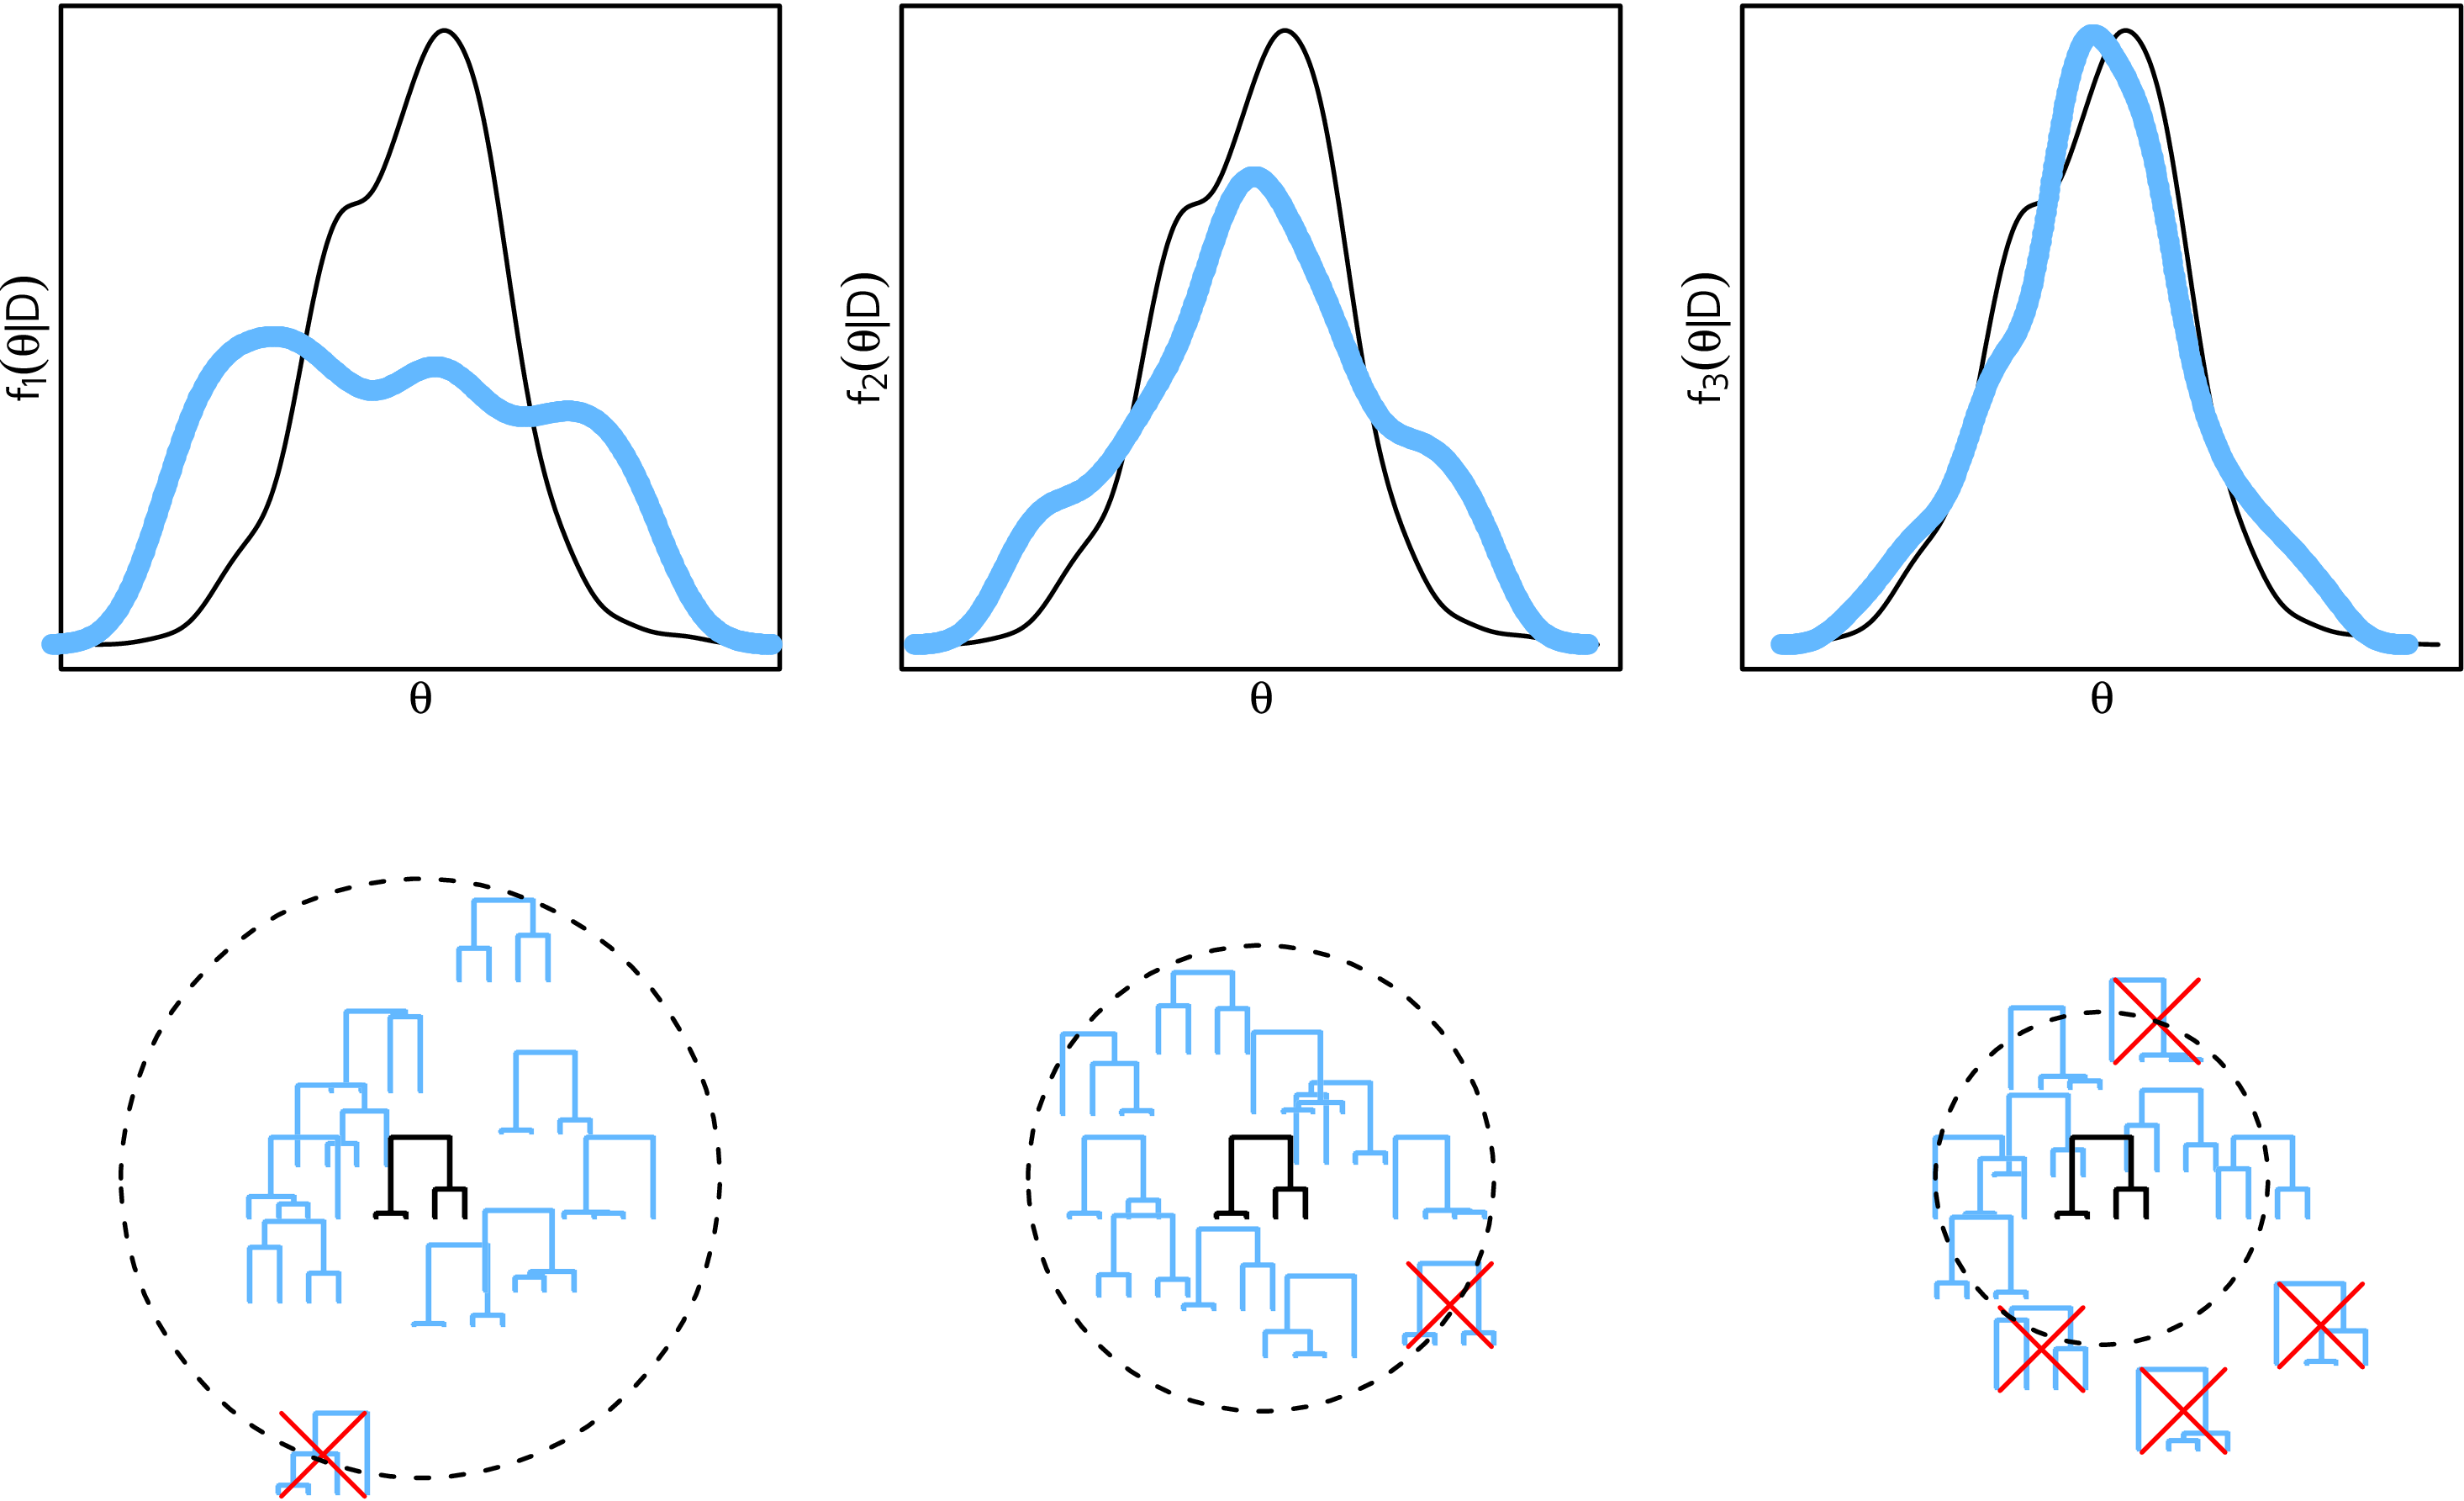
\includegraphics[width=\textwidth]{abc-smc}};
    \only<1>{
      \fill [white] (-5, -3.5) rectangle (-1.8, 0);
    }
    \only<1-2>{
      \fill [white] (-1.8, -3) rectangle (5.5, 3.3);
    }
    \only<3-4>{
      \fill [white] (1.8, -3) rectangle (5.5, 3.3);
    }
    \only<3>{
      \fill [white] (-1.8, 0) rectangle (2, 3.3);
    }
    \only<5>{
      \fill [white] (1.8, 0) rectangle (5.5, 3.3);
    }
    \uncover<7>{
      \node [below=0.2 of a] {\Large sequential Monte Carlo};
    }
  \end{tikzpicture}
\end{frame}
